\PassOptionsToPackage{unicode=true}{hyperref} % options for packages loaded elsewhere
\PassOptionsToPackage{hyphens}{url}
%
\documentclass[]{article}
\usepackage{lmodern}
\usepackage{amssymb,amsmath}
\usepackage{ifxetex,ifluatex}
\usepackage{fixltx2e} % provides \textsubscript
\ifnum 0\ifxetex 1\fi\ifluatex 1\fi=0 % if pdftex
  \usepackage[T1]{fontenc}
  \usepackage[utf8]{inputenc}
  \usepackage{textcomp} % provides euro and other symbols
\else % if luatex or xelatex
  \usepackage{unicode-math}
  \defaultfontfeatures{Ligatures=TeX,Scale=MatchLowercase}
\fi
% use upquote if available, for straight quotes in verbatim environments
\IfFileExists{upquote.sty}{\usepackage{upquote}}{}
% use microtype if available
\IfFileExists{microtype.sty}{%
\usepackage[]{microtype}
\UseMicrotypeSet[protrusion]{basicmath} % disable protrusion for tt fonts
}{}
\IfFileExists{parskip.sty}{%
\usepackage{parskip}
}{% else
\setlength{\parindent}{0pt}
\setlength{\parskip}{6pt plus 2pt minus 1pt}
}
\usepackage{hyperref}
\hypersetup{
            pdftitle={Week3},
            pdfauthor={Thomas Rosenthal},
            pdfborder={0 0 0},
            breaklinks=true}
\urlstyle{same}  % don't use monospace font for urls
\usepackage[margin=1in]{geometry}
\usepackage{color}
\usepackage{fancyvrb}
\newcommand{\VerbBar}{|}
\newcommand{\VERB}{\Verb[commandchars=\\\{\}]}
\DefineVerbatimEnvironment{Highlighting}{Verbatim}{commandchars=\\\{\}}
% Add ',fontsize=\small' for more characters per line
\usepackage{framed}
\definecolor{shadecolor}{RGB}{248,248,248}
\newenvironment{Shaded}{\begin{snugshade}}{\end{snugshade}}
\newcommand{\AlertTok}[1]{\textcolor[rgb]{0.94,0.16,0.16}{#1}}
\newcommand{\AnnotationTok}[1]{\textcolor[rgb]{0.56,0.35,0.01}{\textbf{\textit{#1}}}}
\newcommand{\AttributeTok}[1]{\textcolor[rgb]{0.77,0.63,0.00}{#1}}
\newcommand{\BaseNTok}[1]{\textcolor[rgb]{0.00,0.00,0.81}{#1}}
\newcommand{\BuiltInTok}[1]{#1}
\newcommand{\CharTok}[1]{\textcolor[rgb]{0.31,0.60,0.02}{#1}}
\newcommand{\CommentTok}[1]{\textcolor[rgb]{0.56,0.35,0.01}{\textit{#1}}}
\newcommand{\CommentVarTok}[1]{\textcolor[rgb]{0.56,0.35,0.01}{\textbf{\textit{#1}}}}
\newcommand{\ConstantTok}[1]{\textcolor[rgb]{0.00,0.00,0.00}{#1}}
\newcommand{\ControlFlowTok}[1]{\textcolor[rgb]{0.13,0.29,0.53}{\textbf{#1}}}
\newcommand{\DataTypeTok}[1]{\textcolor[rgb]{0.13,0.29,0.53}{#1}}
\newcommand{\DecValTok}[1]{\textcolor[rgb]{0.00,0.00,0.81}{#1}}
\newcommand{\DocumentationTok}[1]{\textcolor[rgb]{0.56,0.35,0.01}{\textbf{\textit{#1}}}}
\newcommand{\ErrorTok}[1]{\textcolor[rgb]{0.64,0.00,0.00}{\textbf{#1}}}
\newcommand{\ExtensionTok}[1]{#1}
\newcommand{\FloatTok}[1]{\textcolor[rgb]{0.00,0.00,0.81}{#1}}
\newcommand{\FunctionTok}[1]{\textcolor[rgb]{0.00,0.00,0.00}{#1}}
\newcommand{\ImportTok}[1]{#1}
\newcommand{\InformationTok}[1]{\textcolor[rgb]{0.56,0.35,0.01}{\textbf{\textit{#1}}}}
\newcommand{\KeywordTok}[1]{\textcolor[rgb]{0.13,0.29,0.53}{\textbf{#1}}}
\newcommand{\NormalTok}[1]{#1}
\newcommand{\OperatorTok}[1]{\textcolor[rgb]{0.81,0.36,0.00}{\textbf{#1}}}
\newcommand{\OtherTok}[1]{\textcolor[rgb]{0.56,0.35,0.01}{#1}}
\newcommand{\PreprocessorTok}[1]{\textcolor[rgb]{0.56,0.35,0.01}{\textit{#1}}}
\newcommand{\RegionMarkerTok}[1]{#1}
\newcommand{\SpecialCharTok}[1]{\textcolor[rgb]{0.00,0.00,0.00}{#1}}
\newcommand{\SpecialStringTok}[1]{\textcolor[rgb]{0.31,0.60,0.02}{#1}}
\newcommand{\StringTok}[1]{\textcolor[rgb]{0.31,0.60,0.02}{#1}}
\newcommand{\VariableTok}[1]{\textcolor[rgb]{0.00,0.00,0.00}{#1}}
\newcommand{\VerbatimStringTok}[1]{\textcolor[rgb]{0.31,0.60,0.02}{#1}}
\newcommand{\WarningTok}[1]{\textcolor[rgb]{0.56,0.35,0.01}{\textbf{\textit{#1}}}}
\usepackage{graphicx,grffile}
\makeatletter
\def\maxwidth{\ifdim\Gin@nat@width>\linewidth\linewidth\else\Gin@nat@width\fi}
\def\maxheight{\ifdim\Gin@nat@height>\textheight\textheight\else\Gin@nat@height\fi}
\makeatother
% Scale images if necessary, so that they will not overflow the page
% margins by default, and it is still possible to overwrite the defaults
% using explicit options in \includegraphics[width, height, ...]{}
\setkeys{Gin}{width=\maxwidth,height=\maxheight,keepaspectratio}
\setlength{\emergencystretch}{3em}  % prevent overfull lines
\providecommand{\tightlist}{%
  \setlength{\itemsep}{0pt}\setlength{\parskip}{0pt}}
\setcounter{secnumdepth}{0}
% Redefines (sub)paragraphs to behave more like sections
\ifx\paragraph\undefined\else
\let\oldparagraph\paragraph
\renewcommand{\paragraph}[1]{\oldparagraph{#1}\mbox{}}
\fi
\ifx\subparagraph\undefined\else
\let\oldsubparagraph\subparagraph
\renewcommand{\subparagraph}[1]{\oldsubparagraph{#1}\mbox{}}
\fi

% set default figure placement to htbp
\makeatletter
\def\fps@figure{htbp}
\makeatother


\title{Week3}
\author{Thomas Rosenthal}
\date{28/01/2021}

\begin{document}
\maketitle

\hypertarget{weekly-reflection-my-lesson-in-html-node-picking}{%
\subsection{Weekly Reflection, My Lesson in HTML node
picking}\label{weekly-reflection-my-lesson-in-html-node-picking}}

For the past few weeks now, I have been looking to programmatically
navigate from a collections page (think, results in from search on a
webstore) to a specific item's page and extract details from within it.
To do this, a few things have to happen.

For this example, I will use the coffees from
\href{https://www.thelibraryspecialtycoffee.com/}{The Library Speciality
Coffee} on
\href{https://eightouncecoffee.ca/collections/the-library-specialty-coffee}{Eight
Ounce Coffee}. Let's suppose that we want to quickly grab the
\textbf{Altitude} of every coffee. We see that this information isn't
listed in the colletion page.

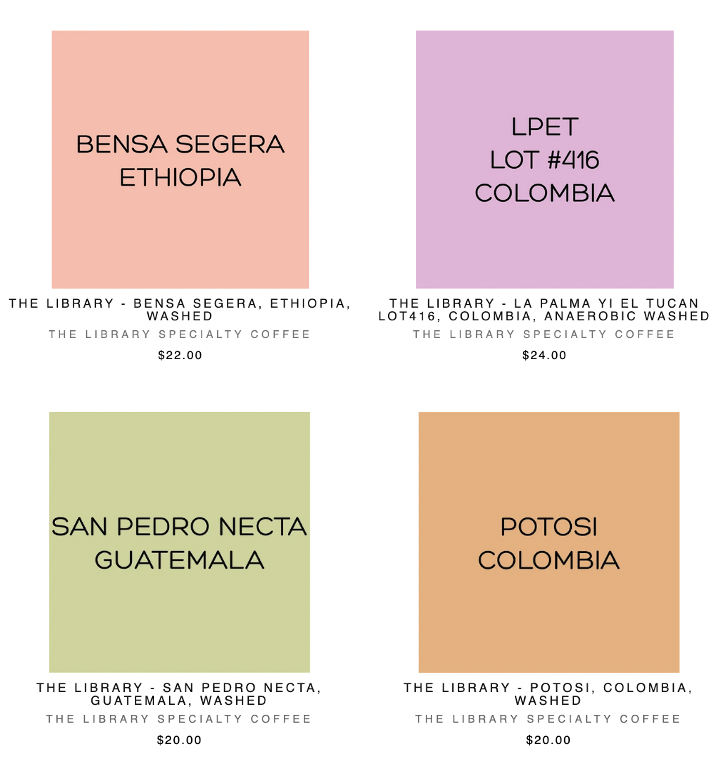
\includegraphics[width=0.3\linewidth]{/Users/thomas/Documents/GitHub/COFEE_COFFEE_COFFEE/journal/Week3/imgs/TLS}

We'll need to navigate to each coffee's page, extract the altitude,
write it to a table (assumedly with the coffee name, region, processing,
etc as well), and then move on to the next coffee and repeat the
process.

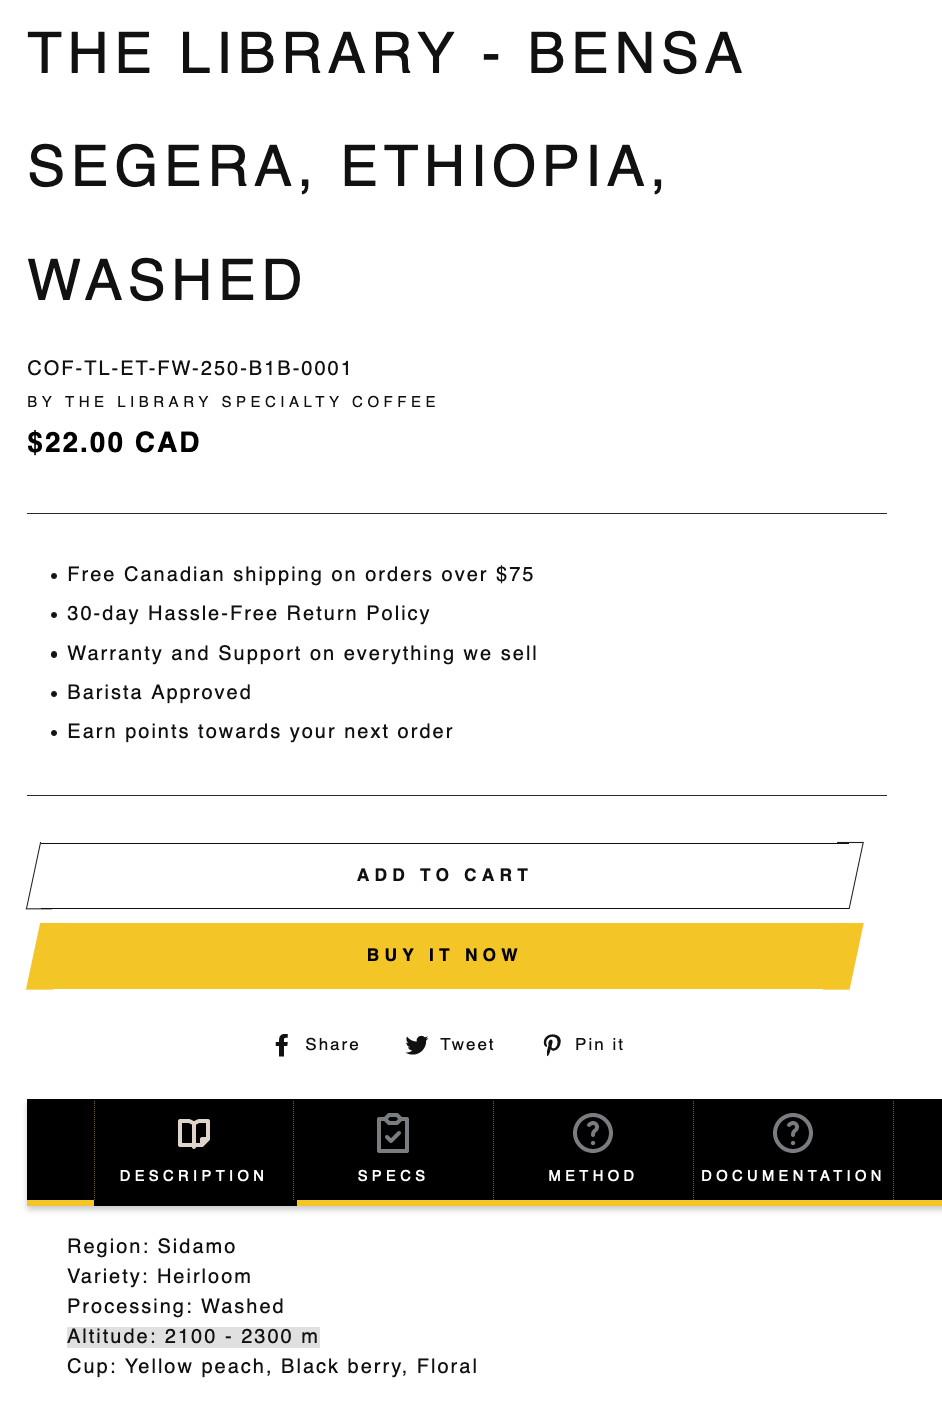
\includegraphics[width=0.35\linewidth]{/Users/thomas/Documents/GitHub/COFEE_COFFEE_COFFEE/journal/Week3/imgs/bensa}

Using
\href{https://blog.rstudio.com/2014/11/24/rvest-easy-web-scraping-with-r/}{rvest},
we'll aim to grab the desired information from a saved html file
(because let's be polite when we're scraping someone else's date).
Depending on the site complexity, this might seem incredibly daunting,
and you might find yourself doing a lot of trial and error to get to
information you want to extract..

\begin{Shaded}
\begin{Highlighting}[]
\KeywordTok{library}\NormalTok{(rvest)}
\end{Highlighting}
\end{Shaded}

\begin{Shaded}
\begin{Highlighting}[]
\NormalTok{raw_data <-}\StringTok{ }\KeywordTok{read_html}\NormalTok{(}\StringTok{"https://eightouncecoffee.ca/collections/the-library-specialty-coffee"}\NormalTok{)}
\KeywordTok{write_html}\NormalTok{(raw_data, }\StringTok{"journal/Week3/inputs/TLS.html"}\NormalTok{) }\CommentTok{# Note that we save the file as a html file}
\end{Highlighting}
\end{Shaded}

Once we have the html file, we'll need to navigate to each coffee.

The page source will start to show us what we are looking for. Here I've
searched for ``Bensa'' just to move through the page a bit quicker.

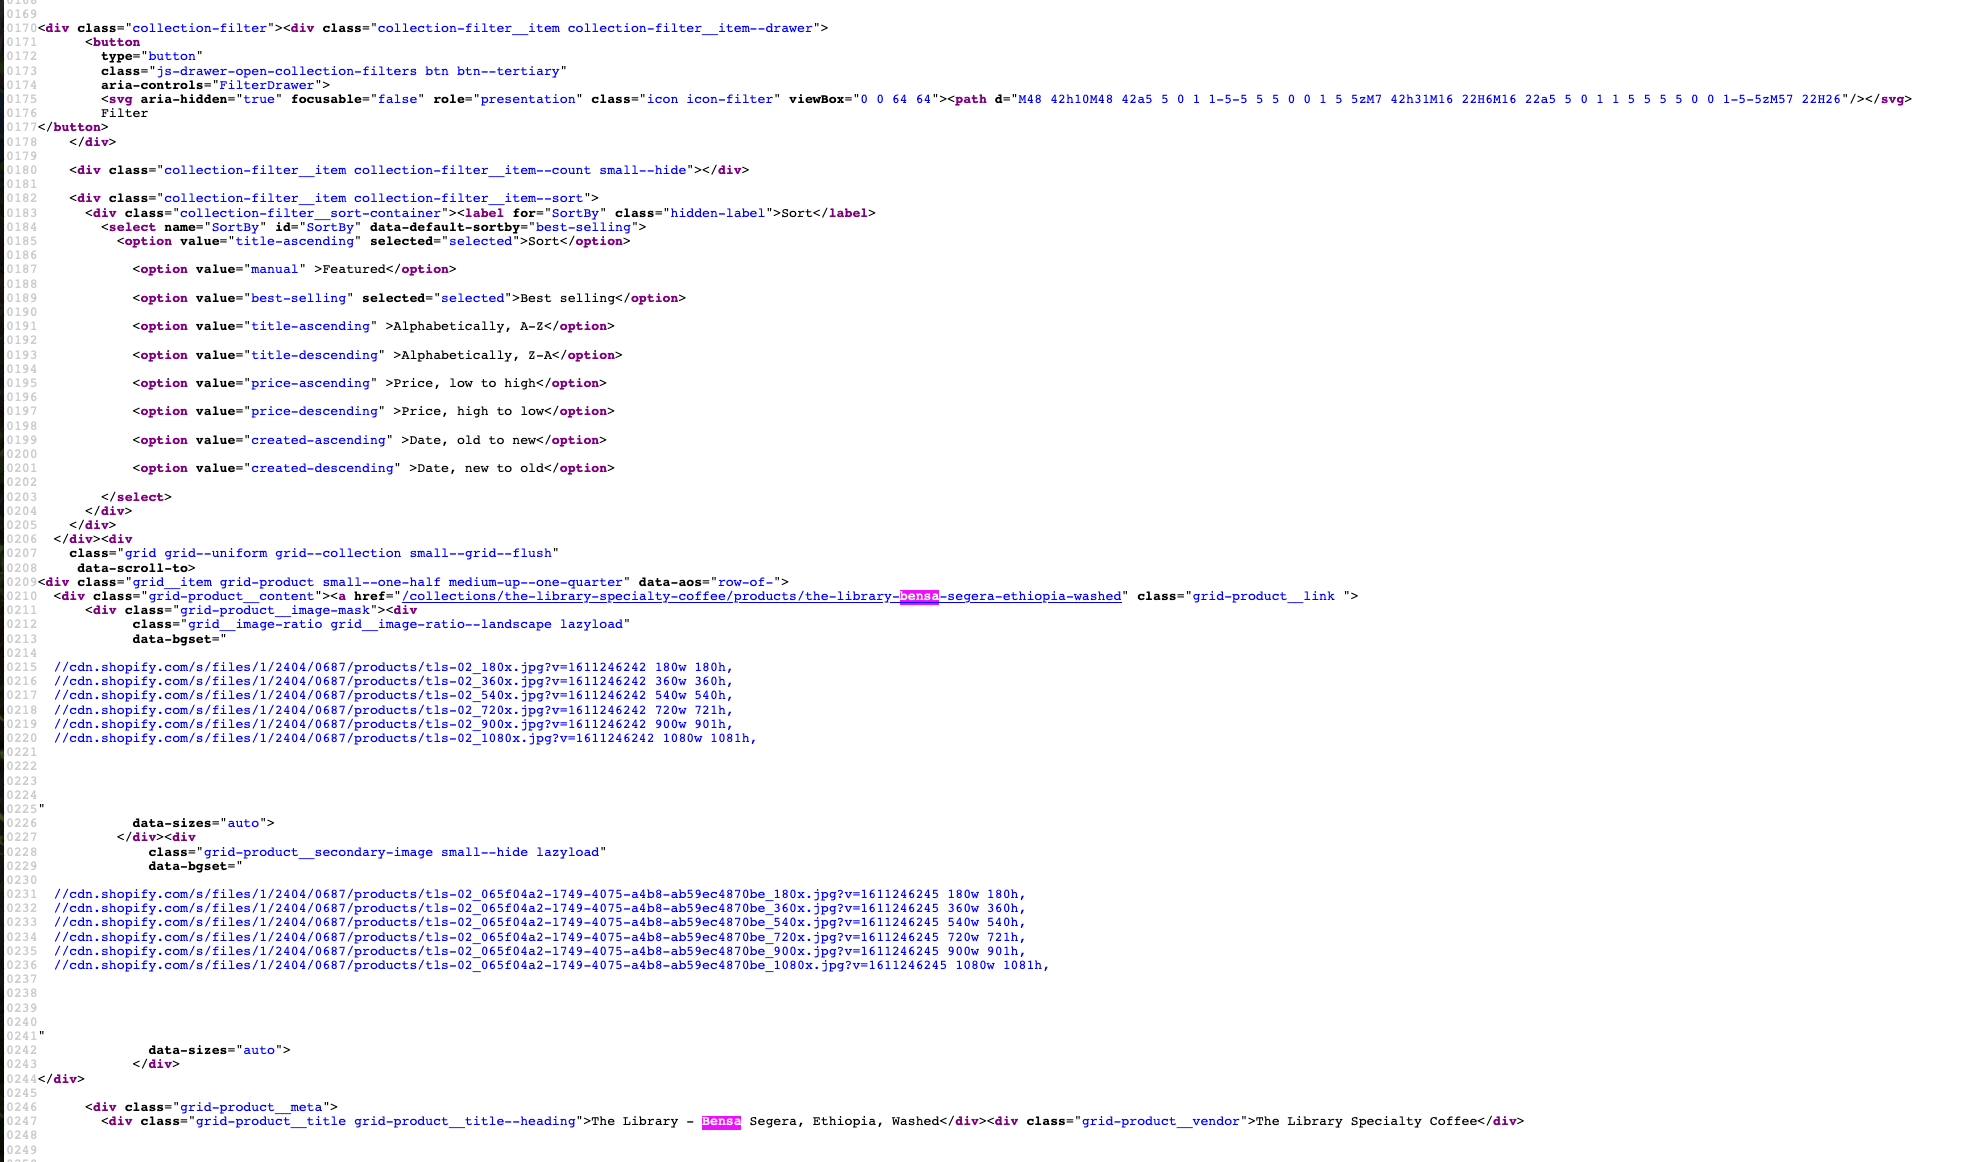
\includegraphics[width=0.75\linewidth]{/Users/thomas/Documents/GitHub/COFEE_COFFEE_COFFEE/journal/Week3/imgs/page-source}

When I first started working with rvest, I thought it was necessary to
traverse an entire html ``tree'' going from one node to another.

It was looking something like this:

\begin{Shaded}
\begin{Highlighting}[]
\KeywordTok{library}\NormalTok{(tidyverse)}
\NormalTok{rough <-}\StringTok{ }\NormalTok{raw_data }\OperatorTok\StringTok{ }
\StringTok{  }\KeywordTok{html_nodes}\NormalTok{(}\StringTok{"body"}\NormalTok{) }\OperatorTok\StringTok{ }
\StringTok{  }\KeywordTok{html_nodes}\NormalTok{(}\StringTok{"div"}\NormalTok{) }\OperatorTok
\StringTok{  }\KeywordTok{html_nodes}\NormalTok{(}\StringTok{"div"}\NormalTok{) }\OperatorTok
\StringTok{  }\KeywordTok{html_nodes}\NormalTok{(}\StringTok{"main"}\NormalTok{) }\OperatorTok
\StringTok{  }\KeywordTok{html_nodes}\NormalTok{(}\StringTok{"div"}\NormalTok{) }\OperatorTok
\StringTok{  }\KeywordTok{html_nodes}\NormalTok{(}\StringTok{"div"}\NormalTok{) }\OperatorTok
\StringTok{  }\KeywordTok{html_nodes}\NormalTok{(}\StringTok{"div"}\NormalTok{) }\OperatorTok
\StringTok{  }\KeywordTok{html_text}\NormalTok{() }
\KeywordTok{tibble}\NormalTok{(}\DataTypeTok{raw_text =} \KeywordTok{head}\NormalTok{(rough[}\DecValTok{46}\OperatorTok{:}\DecValTok{55}\NormalTok{],}\DecValTok{10}\NormalTok{))}
\end{Highlighting}
\end{Shaded}

\begin{verbatim}
## # A tibble: 10 x 1
##    raw_text                                                                     
##    <chr>                                                                        
##  1 "\n\n  \n      \n          \n            \n\n\n      \n        The Library -~
##  2 "\n  \n      \n          \n            \n\n\n      \n        The Library - B~
##  3 "\n      \n          \n            \n\n\n      \n        The Library - Bensa~
##  4 "\n          \n            \n"                                               
##  5 "\n          "                                                               
##  6 "\n            "                                                             
##  7 "\n        The Library - Bensa Segera, Ethiopia, WashedThe Library Specialty~
##  8 "The Library - Bensa Segera, Ethiopia, Washed"                               
##  9 "The Library Specialty Coffee"                                               
## 10 "\n       No reviews  \n"
\end{verbatim}

On a side note, it was possible to just use html\_nodes() once:

\begin{verbatim}
html_nodes("body div div main div div div") %>%
html_text() 
\end{verbatim}

but this is a bit beside the point!

I have filtered this down to exclude a ton of non relevent information
for the sake of this writeup (like the first 45 rows for example), but
this isn't very programmatic. In reality, I ended up writing something
to grab the coffee lines because they had a unique number of
\textbackslash{}n \textbackslash{}n \textbackslash{}n \textbackslash{}n.

\begin{Shaded}
\begin{Highlighting}[]
\KeywordTok{library}\NormalTok{(data.table)}
\NormalTok{some_data <-}\StringTok{ }
\KeywordTok{tibble}\NormalTok{(}\DataTypeTok{raw_text =}\NormalTok{ rough[}\DecValTok{46}\OperatorTok{:}\DecValTok{81}\NormalTok{])}

\NormalTok{some_data <-}\StringTok{ }\NormalTok{some_data }\OperatorTok\StringTok{ }
\StringTok{  }\KeywordTok{mutate}\NormalTok{(}\DataTypeTok{is_TLS =} \KeywordTok{if_else}\NormalTok{(raw_text }\OperatorTok\StringTok{ "}\CharTok{\textbackslash{}n\textbackslash{}n\textbackslash{}n\textbackslash{}n\textbackslash{}n\textbackslash{}n\textbackslash{}n\textbackslash{}n\textbackslash{}n\textbackslash{}n\textbackslash{}n\textbackslash{}n\textbackslash{}n\textbackslash{}n}\StringTok{ "}\NormalTok{,}\DecValTok{1}\NormalTok{,}\DecValTok{0}\NormalTok{)) }\OperatorTok\StringTok{ }
\StringTok{  }\KeywordTok{filter}\NormalTok{(is_TLS }\OperatorTok{==}\StringTok{ }\DecValTok{1}\NormalTok{) }
\NormalTok{some_data}
\end{Highlighting}
\end{Shaded}

\begin{verbatim}
## # A tibble: 12 x 2
##    raw_text                                                               is_TLS
##    <chr>                                                                   <dbl>
##  1 "\n\n  \n      \n          \n            \n\n\n      \n        The Li~      1
##  2 "\n  \n      \n          \n            \n\n\n      \n        The Libr~      1
##  3 "\n      \n          \n            \n\n\n      \n        The Library ~      1
##  4 "\n        The Library - Bensa Segera, Ethiopia, WashedThe Library Sp~      1
##  5 "\n  \n      \n          \n            \n\n\n      \n        The Libr~      1
##  6 "\n      \n          \n            \n\n\n      \n        The Library ~      1
##  7 "\n        The Library - La Palma yi El Tucan lot416, Colombia, Anaer~      1
##  8 "\n  \n      \n          \n            \n\n\n      \n        The Libr~      1
##  9 "\n      \n          \n            \n\n\n      \n        The Library ~      1
## 10 "\n        The Library - San Pedro Necta, Guatemala, WashedThe Librar~      1
## 11 "\n  \n      \n          \n            \n\n\n      \n        The Libr~      1
## 12 "\n      \n          \n            \n\n\n      \n        The Library ~      1
\end{verbatim}

Obviously this wasn't working well -- I end up with a lot of extra data
cleaning, and the number of \textbackslash{}n characters was changing
week by week. Ouch.

Unfortunately, even figuring out that coffee names were appearing every
n-th row isn't particularly programmatic\ldots{}it would change week to
week.

\begin{Shaded}
\begin{Highlighting}[]
\KeywordTok{tibble}\NormalTok{(}\DataTypeTok{raw_text =} \KeywordTok{head}\NormalTok{(rough[}\KeywordTok{c}\NormalTok{(}\DecValTok{53}\NormalTok{,}\DecValTok{64}\NormalTok{,}\DecValTok{75}\NormalTok{,}\DecValTok{86}\NormalTok{)],}\DecValTok{4}\NormalTok{))}
\end{Highlighting}
\end{Shaded}

\begin{verbatim}
## # A tibble: 4 x 1
##   raw_text                                                             
##   <chr>                                                                
## 1 The Library - Bensa Segera, Ethiopia, Washed                         
## 2 The Library - La Palma yi El Tucan lot416, Colombia, Anaerobic washed
## 3 The Library - San Pedro Necta, Guatemala, Washed                     
## 4 The Library - Potosi, Colombia, Washed
\end{verbatim}

\hypertarget{picking-the-right-node}{%
\subsubsection{Picking the Right Node}\label{picking-the-right-node}}

A better solution requires that we go back to the page source.

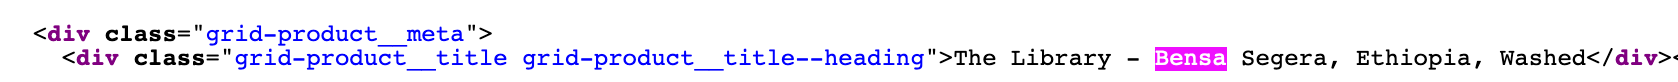
\includegraphics[width=1\linewidth]{/Users/thomas/Documents/GitHub/COFEE_COFFEE_COFFEE/journal/Week3/imgs/class=}

While I was trying to browse through these HTML files with 12000 lines,
I noticed that almost every \textless{}div\textgreater{} had either an
\textbf{id =} or \textbf{class =} within it. Ah ha.

Let's try that instead.

\begin{Shaded}
\begin{Highlighting}[]
\NormalTok{clean <-}\StringTok{ }\NormalTok{raw_data }\OperatorTok\StringTok{ }
\StringTok{  }\KeywordTok{html_nodes}\NormalTok{(}\StringTok{"div [class='grid-product__title grid-product__title--heading']"}\NormalTok{) }\OperatorTok\StringTok{ }
\StringTok{  }\KeywordTok{html_text}\NormalTok{()}
\NormalTok{clean}
\end{Highlighting}
\end{Shaded}

\begin{verbatim}
## [1] "The Library - Bensa Segera, Ethiopia, Washed"                         
## [2] "The Library - La Palma yi El Tucan lot416, Colombia, Anaerobic washed"
## [3] "The Library - San Pedro Necta, Guatemala, Washed"                     
## [4] "The Library - Potosi, Colombia, Washed"
\end{verbatim}

This is great. Not only have we totally forgotten about this

nonsense, we are navigating to a single place on the webpage.

This starts to let us grab every coffee name to generate into a URL. I
noticed early on that coffee names were always the same as the URLs (as
lower case strings with hypens replacing spaces).

Let's make it lowercase with \texttt{str\_to\_lower}

\begin{Shaded}
\begin{Highlighting}[]
\NormalTok{our_data <-}\StringTok{ }\KeywordTok{tibble}\NormalTok{(}\DataTypeTok{raw_text =}\NormalTok{ clean)}

\NormalTok{coffee_names <-}\StringTok{ }\NormalTok{our_data }\OperatorTok\StringTok{ }
\StringTok{  }\KeywordTok{mutate}\NormalTok{(}\DataTypeTok{lower_name =}  \KeywordTok{str_to_lower}\NormalTok{(raw_text)) }\OperatorTok\StringTok{ }
\StringTok{  }\KeywordTok{select}\NormalTok{(lower_name)}
\NormalTok{coffee_names}
\end{Highlighting}
\end{Shaded}

\begin{verbatim}
## # A tibble: 4 x 1
##   lower_name                                                           
##   <chr>                                                                
## 1 the library - bensa segera, ethiopia, washed                         
## 2 the library - la palma yi el tucan lot416, colombia, anaerobic washed
## 3 the library - san pedro necta, guatemala, washed                     
## 4 the library - potosi, colombia, washed
\end{verbatim}

Some substituion will help us here

\begin{Shaded}
\begin{Highlighting}[]
\NormalTok{hypen_names <-}\StringTok{ }\NormalTok{coffee_names }\OperatorTok\StringTok{ }
\StringTok{  }\KeywordTok{apply}\NormalTok{( }\DataTypeTok{MARGIN =} \DecValTok{2}\NormalTok{, }\DataTypeTok{FUN =}\NormalTok{ trimws) }\OperatorTok\StringTok{ }
\StringTok{  }\KeywordTok{sapply}\NormalTok{(gsub, }\DataTypeTok{pattern =} \StringTok{" "}\NormalTok{, }\DataTypeTok{replacement =} \StringTok{"-"}\NormalTok{, }\DataTypeTok{fixed =} \OtherTok{TRUE}\NormalTok{) }\OperatorTok\StringTok{ }
\StringTok{  }\KeywordTok{sapply}\NormalTok{(gsub, }\DataTypeTok{pattern =} \StringTok{","}\NormalTok{, }\DataTypeTok{replacement =} \StringTok{""}\NormalTok{, }\DataTypeTok{fixed =} \OtherTok{TRUE}\NormalTok{) }\OperatorTok
\StringTok{  }\KeywordTok{sapply}\NormalTok{(gsub, }\DataTypeTok{pattern =} \StringTok{"---"}\NormalTok{, }\DataTypeTok{replacement =} \StringTok{"-"}\NormalTok{, }\DataTypeTok{fixed =} \OtherTok{TRUE}\NormalTok{) }\OperatorTok
\StringTok{  }\KeywordTok{as.data.frame}\NormalTok{() }\OperatorTok\StringTok{ }
\StringTok{  }\KeywordTok{rename}\NormalTok{(}\DataTypeTok{Hypen_Name =} \DecValTok{1}\NormalTok{) }

\KeywordTok{rownames}\NormalTok{(hypen_names) <-}\StringTok{ }\DecValTok{1}\OperatorTok{:}\KeywordTok{nrow}\NormalTok{(hypen_names)}
\NormalTok{hypen_names}
\end{Highlighting}
\end{Shaded}

\begin{verbatim}
##                                                          Hypen_Name
## 1                          the-library-bensa-segera-ethiopia-washed
## 2 the-library-la-palma-yi-el-tucan-lot416-colombia-anaerobic-washed
## 3                      the-library-san-pedro-necta-guatemala-washed
## 4                                the-library-potosi-colombia-washed
\end{verbatim}

Now we can just add the collection prefix with paste:
`\url{https://eightouncecoffee.ca/collections/the-library-specialty-coffee/products/}'

\begin{Shaded}
\begin{Highlighting}[]
\NormalTok{URLs <-}\StringTok{ }\KeywordTok{paste0}\NormalTok{(}\StringTok{"https://eightouncecoffee.ca/collections/the-library-specialty-coffee/products/"}\NormalTok{,hypen_names[,}\DecValTok{1}\NormalTok{])}
\NormalTok{URLs[}\DecValTok{1}\NormalTok{]}
\end{Highlighting}
\end{Shaded}

\begin{verbatim}
## [1] "https://eightouncecoffee.ca/collections/the-library-specialty-coffee/products/the-library-bensa-segera-ethiopia-washed"
\end{verbatim}

Within a for-loop, we can easily feed this into another rvest
\texttt{read\_html}, pick the correct \texttt{html\_node()}
\textbf{(USING class= THIS TIME, RIGHT?)} and extract out the alititude
like we wanted.

\begin{Shaded}
\begin{Highlighting}[]
\NormalTok{coffee_table <-}\StringTok{ }\KeywordTok{data.frame}\NormalTok{()}

\CommentTok{#I will just do this for the first coffee}
\ControlFlowTok{for}\NormalTok{(i }\ControlFlowTok{in}\NormalTok{ URLs[}\DecValTok{1}\NormalTok{])\{}
\NormalTok{  coffee_row <-}\StringTok{ }\KeywordTok{read_html}\NormalTok{(i)}
  
\NormalTok{  coffee_details <-}\StringTok{ }
\StringTok{  }\NormalTok{coffee_row }\OperatorTok\StringTok{ }
\StringTok{    }\KeywordTok{html_nodes}\NormalTok{(}\StringTok{"div [id='content'] ul li p"}\NormalTok{) }\OperatorTok\StringTok{ }
\StringTok{    }\KeywordTok{html_text}\NormalTok{()}
  
  \CommentTok{#write it out so you can use it again!}
  \KeywordTok{write_html}\NormalTok{(coffee_row,}\KeywordTok{paste0}\NormalTok{(}\StringTok{"journal/Week3/inputs/coffee.html"}\NormalTok{))}
  
\NormalTok{  coffee <-}\StringTok{ }\KeywordTok{tibble}\NormalTok{(}\DataTypeTok{raw_text =}\NormalTok{ coffee_details)}
  
  \CommentTok{#seperate details row into relevent columns}
\NormalTok{  coffee <-}\StringTok{ }\NormalTok{coffee }\OperatorTok
\StringTok{    }\KeywordTok{pivot_wider}\NormalTok{(}\DataTypeTok{names_from =} \DecValTok{1}\NormalTok{, }\DataTypeTok{values_from =}\NormalTok{ raw_text) }\OperatorTok\StringTok{ }
\StringTok{    }\KeywordTok{rename}\NormalTok{(}\DataTypeTok{table =} \DecValTok{1}\NormalTok{) }\OperatorTok\StringTok{   }
\StringTok{    }\KeywordTok{separate}\NormalTok{(table, }\DataTypeTok{into =} \KeywordTok{c}\NormalTok{(}\StringTok{"1"}\NormalTok{,}\StringTok{"Region"}\NormalTok{,}\StringTok{"Variety"}\NormalTok{,}\StringTok{"Processing"}\NormalTok{,}\StringTok{"Altitude"}\NormalTok{, }\StringTok{"TastingNotes"}\NormalTok{), }\DataTypeTok{sep =} \StringTok{"}\CharTok{\textbackslash{}\textbackslash{}}\StringTok{w+:"}\NormalTok{,  }\DataTypeTok{remove =} \OtherTok{TRUE}\NormalTok{) }\OperatorTok\StringTok{ }
\StringTok{    }\KeywordTok{select}\NormalTok{(}\StringTok{"Region"}\NormalTok{,}\StringTok{"Variety"}\NormalTok{,}\StringTok{"Processing"}\NormalTok{,}\StringTok{"Altitude"}\NormalTok{, }\StringTok{"TastingNotes"}\NormalTok{)  }
    
\CommentTok{#append to a table  }
  \ControlFlowTok{for}\NormalTok{ (i }\ControlFlowTok{in} \KeywordTok{nrow}\NormalTok{(coffee)) \{}
\NormalTok{      coffee_table <-}\StringTok{ }\KeywordTok{rbind}\NormalTok{(coffee_table, }\KeywordTok{data.frame}\NormalTok{(coffee))}
\NormalTok{  \}}
  \CommentTok{#this is a nice little polite pause during loops!}
  \KeywordTok{Sys.sleep}\NormalTok{(}\FloatTok{2.5}\NormalTok{)}
\NormalTok{\}}
\NormalTok{coffee_table}
\end{Highlighting}
\end{Shaded}

\begin{verbatim}
##     Region    Variety Processing        Altitude
## 1  Sidamo   Heirloom     Washed   2100 - 2300 m 
##                         TastingNotes
## 1  Yellow peach, Black berry, Floral
\end{verbatim}

There we have it. Our Altitude is \emph{2100-2300 m} just what we
expected.

\hypertarget{using-html_attr-instead}{%
\subsubsection{Using html\_attr()
instead\ldots{}}\label{using-html_attr-instead}}

So it works. Great. But there's a problem with this approach. It
requires:

\begin{enumerate}
\def\labelenumi{\arabic{enumi})}
\tightlist
\item
  coffee names to be the same as their URLs (or at least some
  discernable pattern)
\item
  coffee names to be free of typos.
\end{enumerate}

That last point seemed like it wouldn't happen. But I found out pretty
quickly that I was wrong.

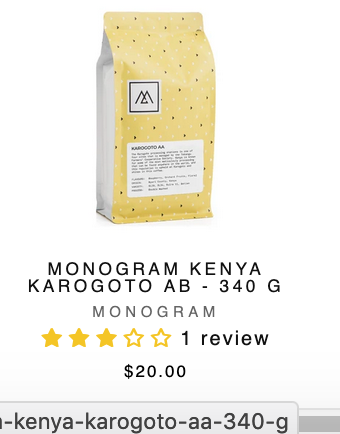
\includegraphics[width=0.25\linewidth]{/Users/thomas/Documents/GitHub/COFEE_COFFEE_COFFEE/journal/Week3/imgs/typo}

It might be hard to notice what's happening here, but AB should have
been AA (AA and AB are Kenyan grades, this isn't overly important, but
maybe you were wondering!)

We can write a fuction to remove them:

\begin{verbatim}
checkURLs <- lapply(URLs, function(u) {
  tryCatch({
    html_obj <- read_html(u)
    draft_table <- html_nodes(html_obj,'table')
    cik <- substr(u,start = 41,stop = 47)
    draft1 <- html_table(draft_table,fill = TRUE)
    final <- u
  }, error = function(x) NULL)
})
\end{verbatim}

but there's a better solution entirely. Exract the URL specifically
using \texttt{html\_attr} rather than \texttt{html\_text}.

While digging around in the page source, I noticed that the URL was
already listed:

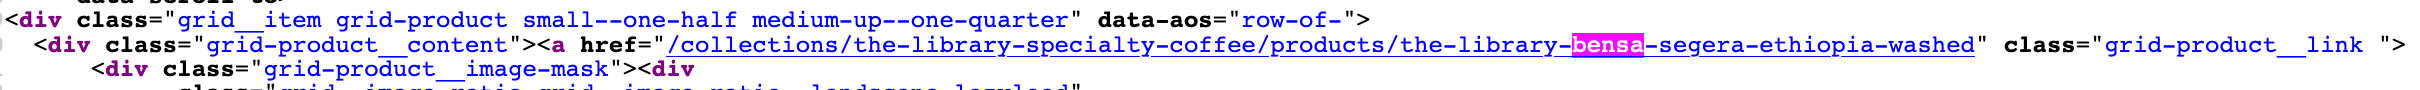
\includegraphics[width=1\linewidth]{/Users/thomas/Documents/GitHub/COFEE_COFFEE_COFFEE/journal/Week3/imgs/href=}

So immediately I tried to grab that with class = grid-product\_\_link

\begin{Shaded}
\begin{Highlighting}[]
\NormalTok{url <-}\StringTok{ }\NormalTok{raw_data }\OperatorTok\StringTok{ }
\StringTok{  }\KeywordTok{html_nodes}\NormalTok{(}\StringTok{"div [class='grid-product__content'] a [class='grid-product__link ']"}\NormalTok{) }\OperatorTok\StringTok{ }
\StringTok{  }\KeywordTok{html_text}\NormalTok{()}
\NormalTok{url}
\end{Highlighting}
\end{Shaded}

\begin{verbatim}
## character(0)
\end{verbatim}

No dice. This is where \texttt{html\_attr} comes in.

\begin{Shaded}
\begin{Highlighting}[]
\NormalTok{url <-}\StringTok{ }\NormalTok{raw_data }\OperatorTok\StringTok{ }
\StringTok{  }\KeywordTok{html_nodes}\NormalTok{(}\StringTok{"div [class='grid-product__content'] a"}\NormalTok{) }\OperatorTok\StringTok{ }
\StringTok{  }\KeywordTok{html_attr}\NormalTok{(}\StringTok{"href"}\NormalTok{)}
\NormalTok{url}
\end{Highlighting}
\end{Shaded}

\begin{verbatim}
## [1] "/collections/the-library-specialty-coffee/products/the-library-bensa-segera-ethiopia-washed"                         
## [2] "/collections/the-library-specialty-coffee/products/the-library-la-palma-yi-el-tucan-lot416-colombia-anaerobic-washed"
## [3] "/collections/the-library-specialty-coffee/products/the-library-san-pedro-necta-guatemala-washed"                     
## [4] "/collections/the-library-specialty-coffee/products/the-library-potosi-colombia-washed"
\end{verbatim}

We've picked the right html\_node with class=, and then asked for the
href= and ended up with our URLs.

Everything is the same from here. But our Kenyan AA ≠ Kenyan AB problem
is no more. We've asked for the URL directly from the webpage, rather
than extrapolating the name to URL pattern and replace all the spaces
with hyphens instead.

\end{document}
